\section{새 연구 결과와 물리적 귀결}
\label{sec:results}
현재 연구 단위는 PHYS16에서 열린 \texttt{HH\_DEFECT\_PARAMETER\_RESPONSE}를 수행한다. $\lambda$는 원 HH source의 세기, $b$는 같은 birth packet의 세기다. 두 매개변수는 각 단계마다 같은 값을 갖는다. 열에너지 좌표는 $w\,[\mathrm{eV/H}]$, $f_2$는 endpoint에서 보존된 정확한 $n_{\rm He}/n_{\rm H}$ 비이며,
\[
g=(x_{\rm HII},y_{\rm HeII},y_{\rm HeIII},w)^T,\qquad
d=g_2-g_F,\qquad d_e=(1,f_2,2f_2,0)d
\]
로 정의한다. 원 $\alpha$를 고정한 채 $\lambda$ 또는 $b$만 미분한다. 시간은 $h=625000000\,\mathrm s$, $t_0=160000000000\,\mathrm s$, 두 half의 최종 시각은 $t_2=161250000000\,\mathrm s$다.

\begin{table}[htbp]\centering\scriptsize
\caption{같은 전역 매개변수에 대한 실제 endpoint 결함의 1차 응답. 두 열은 각각 단위 무차원 매개변수당 값이다.}\label{tab:responses}
\setlength{\tabcolsep}{3pt}\begin{tabular}{lll}\toprule
관측량 & $\partial_\lambda$ 포함 & $\partial_b$ 포함\\\midrule
수소 이온화 차이 $d_{x,\theta}$ & $[1.366697436231,1.689925910794]\times10^{-13}$ & $[-3.127854741570,-2.993844665600]\times10^{-9}$\\
He II 차이 $d_{y,\theta}$ & $[5.928617637399,9.956711152243]\times10^{-17}$ & $[1.608398971389,2.774242695334]\times10^{-15}$\\
He III 차이 $d_{z,\theta}$ & $[4.796181447457,6.313426646227]\times10^{-18}$ & $[4.434566279600,4.807180040710]\times10^{-16}$\\
열에너지 차이 [eV/H] $d_{w,\theta}$ & $[-1.686607512876,-1.370408263621]\times10^{-12}$ & $[-3.253014902391,-3.107335579349]\times10^{-10}$\\
전자 수 차이 [H당] $d_{e,\theta}$ & $[1.366754605418,1.690019031785]\times10^{-13}$ & $[-3.127854534459,-2.993844355539]\times10^{-9}$\\
온도 차이 [K] $\Delta T_\theta$ & $[-1.009599125635,-0.8137506081166]\times10^{-8}$ & $[6.776348385589,7.185335549648]\times10^{-5}$\\
\bottomrule\end{tabular}\end{table}


표의 구간은 \texttt{run02}의 실제 외측 결과이며, 매개변수 직사각형 전체를 포함한다. 두 gas 좌표의 경우 상관식을 사용한 구간 폭의 개선은 $\lambda$의 $d_x$에서 약 $1.04\times10^4$배, $d_w$에서 약 $1.44\times10^4$배다. $b$의 해당 두 좌표에서는 각각 약 $42.5$배와 $41.3$배다. 비교 대상은 동일한 이전 $g_{2,\theta}$와 $g_{F,\theta}$ 포함을 독립적으로 뺀 상자다. 이 수치는 새 sample이나 fitting 대신 기존 입력 사이의 정확한 관계를 유지한 효과를 나타낸다.\cite{app17}

\subsection{두 매개변수의 작용}
$\partial_\lambda d_x>0$, $\partial_\lambda d_w<0$이므로 HH 세기를 높이면 두 half와 Full 사이의 추가 이온화 차이가 커지고 열에너지 차이는 더 음수가 된다. 유한 온도 분모의 변화까지 포함한 $\partial_\lambda\Delta T$도 음수다. 반면 $\partial_bd_x<0$, $\partial_bd_w<0$인데도 $\partial_b\Delta T>0$이다. 온도 응답의 정확한 식에서 입자 수 차이에 곱해지는 항이 함께 작용하기 때문이다. 에너지 성분만의 부호로 온도 응답을 대신하지 않고, 뒤의 공통 covector가 두 효과를 같은 분모에서 결합한다.

PHYS16의 $\Delta T\in[-1.585967387181453,-1.210819969055199]\times10^{-3}\,\mathrm K$는 현재 입력으로 재사용된다. 따라서 $b$를 키우면 이 음의 결함을 줄이고, $\lambda$를 키우면 조금 더 크게 만든다. 각 축의 단위 변화에 대한 전역 적분 포함은 그림~\ref{fig:finite}에 보였다. 같은 고정 $\alpha$와 같은 다른 매개변수에서 기준점으로부터의 변화를 나타내는 외측 영역이다.\cite{phys16,app17}

\begin{figure}[htbp]
\centering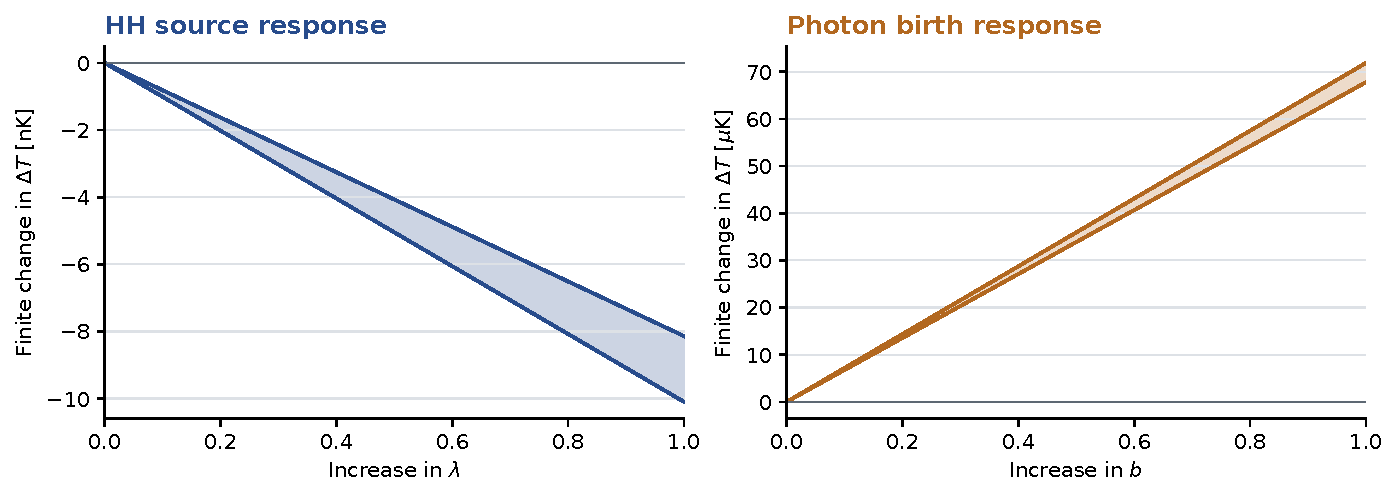
\includegraphics[width=\textwidth]{finite_parameter_envelopes.pdf}
\caption{실제 1차 응답 포함을 적분한 유한 변화 영역. 왼쪽은 $\lambda$ 변화에 따른 감소를 nK 단위로, 오른쪽은 $b$ 변화에 따른 증가를 $\mu$K 단위로 나타낸다. 채색 영역은 모든 동일 계열의 변화에 대한 외측 포함이다. 아래쪽 좌표의 0은 각 비교의 동일 계열 기준점이다.}
\label{fig:finite}
\end{figure}
